\documentclass[hidelinks,12pt]{article}
\usepackage[pdftex]{color, graphicx}
\usepackage{amsmath, amsfonts, amssymb, mathrsfs}
%\usepackage{dcolumn}
\usepackage{natbib}
\usepackage{fancyvrb}
\usepackage{hyperref}
%\usepackage{caption}
%\usepackage{subcaption}
%\usepackage{pdfpages}
\usepackage{lscape}
%\usepackage{hangcaption}
\usepackage{multirow}
\bibpunct{(}{)}{;}{a}{}{,}

\oddsidemargin=0.25in
\evensidemargin=0.25in
\textwidth=6in
\textheight=9.5in
\topmargin=-1in
\footskip=0.5in

\date{}
\author{Wenyu Gao \& Danni Lu \\ Department of Statistics, Virginia Tech}
\title{STAT 5544 Spatial Analysis Final Project \\ (Fall 2016) \\ Spatial Pattern of Population Movement Using Cellular Data }

\begin{document}
	\maketitle
	
	\begin{abstract}
		As increasing number of people are living in urban area, rising issue such as deteriorating periodical traffic congestion in central business districts is gaining more and more attention. The fundamental question to alleviate traffic congestion in urban area is to figure out where the population origins and how population moves spatially. In this report, we applied a spatiotemporal model to analyze the characteristics of population density in metropolitan based on cellular data. Specifically, taking Shanghai as a case study, the spatial and temporal pattern of population density was discussed. Different spatial models were fitted and compared. Predictions were made based on selected models and the results are displayed in choropleth map. The population movement pattern is discussed based on the map. Results show that during the morning peak hours, population move from all over the city to central areas. Areas with relative high population density expand, grow and converge along transportation corridors. 
	\end{abstract}
	\textbf{ {\em Key words}: Cellular Data, Periodical Traffic, Population Movement, Spatial Analysis.}
	
	\section{Introduction}\label{sec:intro}
	Worldwide, urban population has been growing steadily during the past decades, from 33.56\% of the world’s population in 1960 to 53.86\% in 2015. In developed country, the proportion is even higher. 82\% of total population in United States was from urban area in 2015(World Bank, 2015). As increasing number of people are living in urban area, the rising issues such as limited land resource and deteriorating recurrent traffic congestion are repeatedly emphasized by transportation planning institutes. One of the major causes of recurrent traffic congestion is high intensity development in districts where the traffic attraction exceeds the accommodation volume of traffic system. Central Business District (CBD) is therefore becoming the key area to congestion solution as it has been bringing remarkable pressure to transportation system during peak hours in weekday due to their high traffic attraction (Willett K, 2006). 
	
	Central Business District (CBD) is a major destination for urban area. According to a traffic survey of 63 cities in US in the 1950s, about one in every five metropolitan residents has at least one destination in the CBD during each weekday (Foley D L, 1952). Integration of multiple services within a small area is convenient not only for people living in the vicinity but also for people living elsewhere in the city. However, the price to pay is that area with higher developing density requires transportation system with larger capacity during peak hours (Mindali O, 2004), especially in big metropolitan like New York, Sydney and Shanghai. As a consequence, traffic congestion in CBD areas has become a bottleneck for every growing metropolitan to serve better city life.
	
	Researchers have been seeking for solutions to alleviating recurrent traffic congestion for years. Sufficient work has been done on analyzing spatial and temporal characteristic of travel behavior during peak hours. Traditional method to acquire travel pattern information is to conduct household survey, which is usually inefficient and expensive. Nowadays, high density of cellular towers and deep penetration of wireless service provides us with detailed travel information with high accuracy in precise timings. Previous studies have shown a promising future of mobile data in exploring commuting traffic. Compared with traditional way of exploring travel pattern, cellular data stands out for wider coverage area, better representative of population with all kinds of travel pattern, and more detailed information with high accuracy and precise timing. Thus, cellular data allows us to study temporal and spatial travel characteristics of higher graininess. 
	
	Midtown in Shanghai is one of the largest central business districts in the world, which makes it a suitable place to study travel pattern related to CBD. Based on cellular data collected in Shanghai, we’re going to discuss spatial and temporal characteristics of travel pattern related to CBD in Shanghai. In this study, we treat the study area as a continuous field. In section 1, we give a brief introduction of our data, the goal of our study, and make some exploratory analysis to prepare spatial data for modeling. In section 2, we introduce the methodology adopted to build, evaluate and apply the spatial models we fit. In section 3, we demonstrate and discuss the results of our empirical study, model fitting and prediction. At last, conclusions are drawn from the results and discussion. 	
	
	\section{Data Description}\label{sec:data}
We collected geodetic position information of all users in Shanghai from China Mobile for a continuous 24-hour period. China Mobile is the biggest carrier in China, with 64\% total ownership in China (China Mobile, China Unicom and China Telecom, 2016). The dataset includes coded mobile phone ID, date, time, latitude and longitude of corresponding cellular tower. Cellular towers are infrastructure that enables voice and data services for mobile phones. They operate in different radio frequencies, and allow users to maintain their connections while traveling from one base station to another. In total, we collected more than 1.1 billion cell tower hands-off records. These records are from 37,450 different cell towers all over Shanghai with average density of 5.91 cell tower per kilometer square.

One issue of adopting cellular data is privacy of participants (Steenbruggen, John, 2013). To protect their privacy, all records are anonymized and replaced by an identifier ID before we got access to it. In addition, records were aggregated by areal unit and time period before analyzing and visualizing. No personal information is involved and displayed in the research.

The spatial pattern of population density has a direct relationship with traffic demand.  Every morning on weekday, metropolitan sees a population movement from every corner of the city to CBD areas. During peak hours, the traffic on roads and crowding transport is at its highest. The huge increment of population brings tremendous pressure to transportation system near CBD areas. In traditional traffic survey, no standard areal definition of CBD was followed (Foley D L., 1952). Though the importance of CBD in transportation is self-evident, it is much more of a general concept in transportation study. Luckily, the comprehensive information of cellular data provides us a way to identify CBD by its transportation characteristics. In this study, we focus on main districts that are circled by Outer Expressway in Shanghai (Figure \ref{fig:area}).
	\begin{figure}[!ht]
		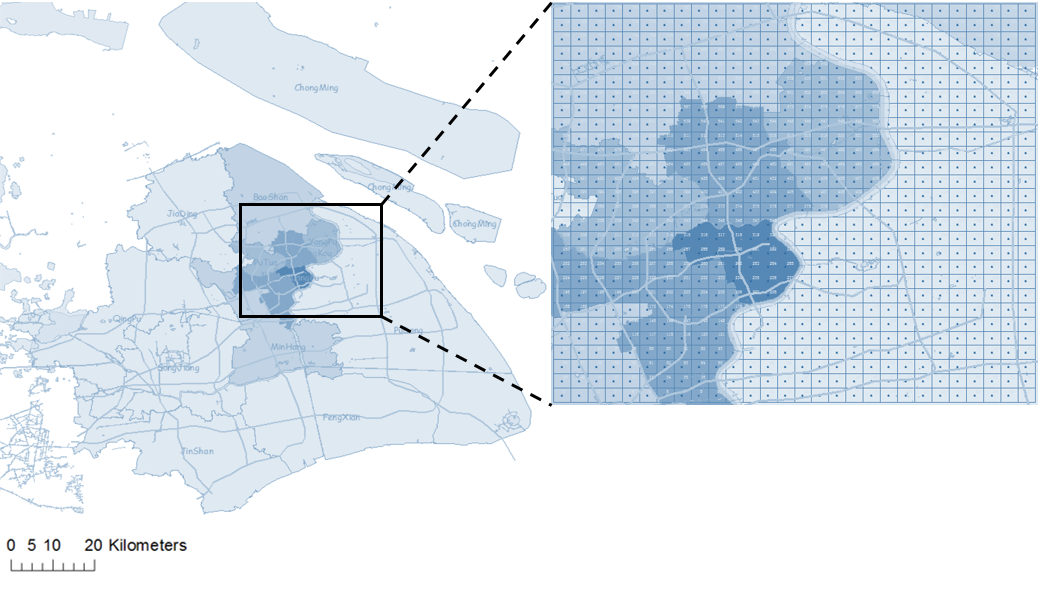
\includegraphics[width=\textwidth]{area.png}
		\caption{Study Area and Aggregation Grid \label{fig:area}}
	\end{figure}
	The accuracy of location information we get depends on the density of cell towers. Instead of accurate location of mobile phone users, cellular data recorded location of cell tower that is nearest to the mobile phone users. As we can see in Figure \ref{fig:tower}, cell towers are not evenly spaced. The density in the center area is higher than outer areas. As a result, the coverage area of each cellular tower is different. To simplify the situation, study area is partitioned into a 28*28 grid, each areal unit is one square kilometer. All cellular information from one areal unit is aggregated into one fictional cell tower in the geo-center of the areal unit (Figure \ref{fig:tower}). Hence, we have a regular point-referenced data to establish spatial model. In terms of study period, our goal is exploring spatial and temporal pattern of population in rush hours in the morning. Previous study shows typical morning rush hours for metropolitan CBDs are between 7:00 and 9:00 am. Therefore, we extract cellular data from 5:00 am to 10:00 am to cover this range.
	\begin{figure}[!ht]
		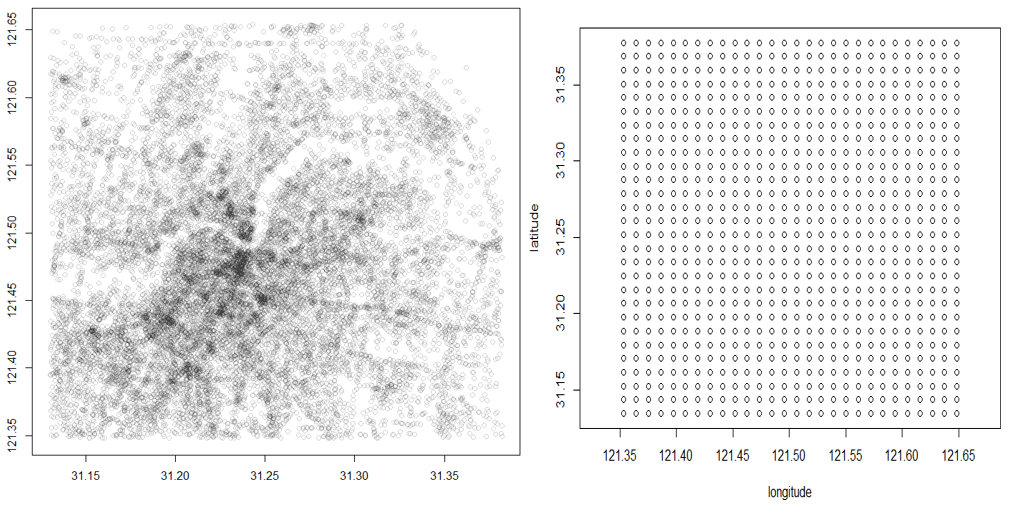
\includegraphics[width=\textwidth]{tower.png}
		\caption{Original Cell Towers and Aggregated Cell Towers \label{fig:tower}}
	\end{figure}
	
	\section{Methodologies}\label{sec:meth}
	Based on our data characteristics and aggregation methods, we treat our data as point-referenced data and apply the corresponding spatial theories for analysis. The whole analyzing process is as follows: We begin from exploratory analysis to check if there is any special structure of the data. Then followed by identification of spatial trend. We would like to analyze the data without spatial trends because this will reflect the intrinsic covariance structure of the data. After detrending, we will check for existence of anisotropy. Model fitting will be conducted after all these preliminary work has been done. Semivariogram fitting and likelihood fitting models are considered. Some model selection criteria are applied to select the best fit and predicted model. Last but not least, we will make inference on the predicted models.
	
	\subsection{Preliminary Analysis}
	Most of the preliminary checks are based on visualization, except for spatial trend detection, where model fitting is conducted. The trend is mainly diagnosed with coordinates.
	\subsection{Model Fitting}
	When plotting the semivariogram, the plot is not reliable if the distance is too large. In data preparation, we aggregated the data to a square of 28km by 28km, indicating that the largest distance is the diagonal line. However, as people are more concentrated in the center, the distance of interest should not be too large. Thus in the following model fitting, we select the largest distance to be around half of the edges, i.e 14 km.
	\subsection{Prediction}
	Model selection for best predicted model is conducted by both visualization and residual sum of squares comparison. Predicted images are based on predicted values at the interpolated points when plotting image for true data rather than the recorded places of true data in the study area. Thus we can compare the predicted models to the true data. 
	
	\section{Results}\label{sec:res}
	\subsection{Exploratory Data Analysis}\label{sec:reseda}
	We begin with a summary table of the dataset, shown in Table \ref{tbl:sumdata}.
	% latex table generated in R 3.3.1 by xtable 1.8-2 package
	% Mon Dec 05 20:09:50 2016
	\begin{table}[ht]
		\centering
		\caption{Summary Table of Dataset \label{tbl:sumdata}}
		\begin{tabular}{rllll}
			\hline
			&      FID &      long &      lat &      freq  \\ 
			\hline
			1 & Min.   :  0.0   & Min.   :121.4   & Min.   :31.13   & Min.   :    0     \\ 
			2 & 1st Qu.:195.8   & 1st Qu.:121.4   & 1st Qu.:31.20   & 1st Qu.: 2060     \\ 
			3 & Median :391.5   & Median :121.5   & Median :31.26   & Median : 5894    \\ 
			4 & Mean   :391.5   & Mean   :121.5   & Mean   :31.26   & Mean   : 9773      \\ 
			5 & 3rd Qu.:587.2   & 3rd Qu.:121.6   & 3rd Qu.:31.32   & 3rd Qu.:14575    \\ 
			6 & Max.   :783.0   & Max.   :121.6   & Max.   :31.38   & Max.   :83822      \\ 
			\hline
			 &    D2Metro &     D2Road &      hour &\\
			\hline
			1  & Min.   :   0.395 & Min.   :   2.274   & Min.   :5 &\\
			2    & 1st Qu.: 387.974  & 1st Qu.: 397.764   & 1st Qu.:6 & \\
			3   & Median : 973.144  & Median : 888.332   & Median :7 &\\
			4  & Mean   :1373.922 & Mean   :1126.451   & Mean   :7 &\\
			5   & 3rd Qu.:1981.959 & 3rd Qu.:1609.672   & 3rd Qu.:8  &\\
			6   & Max.   :6852.305 & Max.   :5607.713   & Max.   :9 & \\
			\hline
		\end{tabular}
	\end{table}
	From the table, it is clear to see that the locations do not vary greatly in longitude and latitude. The frequency, distance to Metro and distance to road have large range and do not seem to be symmetric. There seems no problematic data. We then focus on the frequency variable and we will check the image plot (Figure \ref{fig:image}), perspective plot (Figure \ref{fig:perp} in Appendix \ref{sec:appa}), histogram (Figure \ref{fig:hist}), boxplot (Figure \ref{fig:boxplot} in Appendix \ref{sec:appa}) and qqplot (Figure \ref{fig:qq} in Appendix \ref{sec:appa}) on the variable. Due to page limitation, we only present the image plot and histograms in the paper. The other plots are put to appendices.
	\begin{figure}[!ht]
		\includegraphics[width=\textwidth]{image.png}
		\caption{Image Plots of Frequency by Hour \label{fig:image}}
	\end{figure}
	\begin{figure}[!ht]
		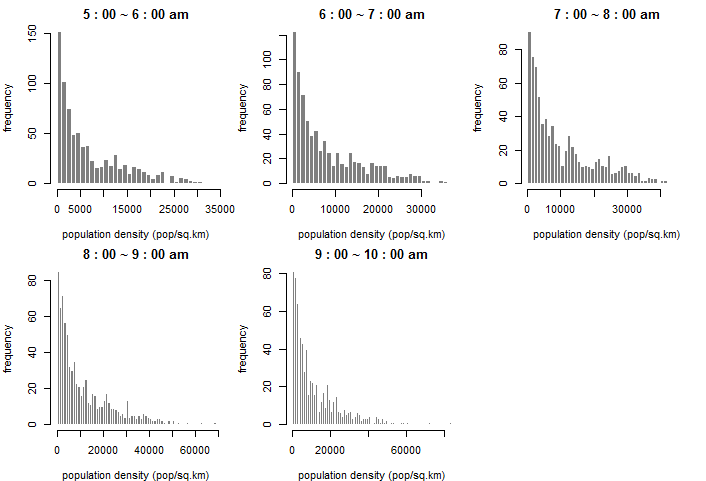
\includegraphics[width=\textwidth]{hist.png}
		\caption{Histograms of Frequency by Hour \label{fig:hist}}
	\end{figure}
	\begin{figure}[!ht]
		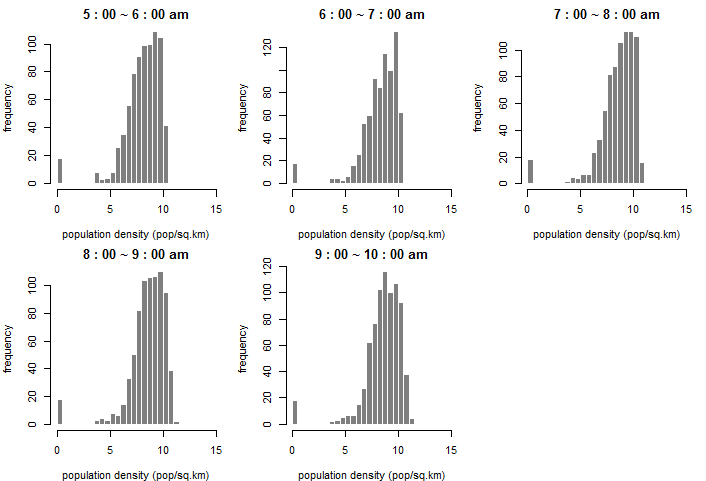
\includegraphics[width=\textwidth]{hist_log.png}
		\caption{Histograms of log-Frequency by Hour \label{fig:lghist}}
	\end{figure}

	Image plots are set to be the same scales where dark red color represents low values while bright yellow colors indicate high values. It is clear that bright colors are centered in the middle and the color becomes brighter and brighter by time. That is, more people are gathering to CBD by time.
	
<<<<<<< HEAD
	Histograms show that frequency is highly skewed. However, after log transformation, the histograms are still not desirable (shown in Figure \ref{fig:lghist}). Similarly, boxplot and qqplot also show that variable frequency does not follow normal distribution. After log transformation, it is still not normally distributed. From the histograms, we can see that frequency is in exponential shape with even steeper slope. A Gamma distribution may be more appropriate. A log transformation may not be very helpful.
	
	For the two covariates, they are also exponentially distributed. This indicates that more people are concentrated near metro lines and expressways.
	\begin{figure}[!ht]
		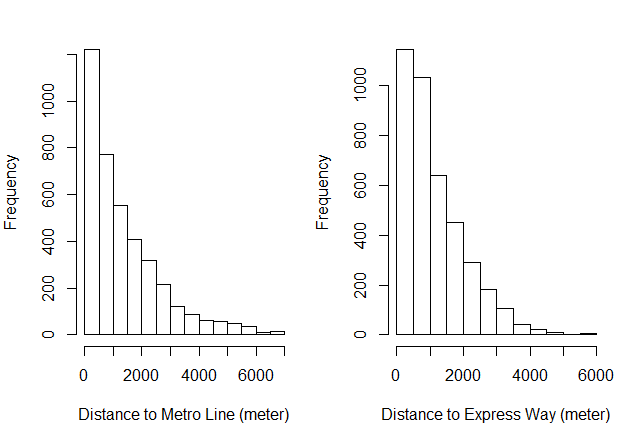
\includegraphics[width=\textwidth]{hist_x.png}
		\caption{Histograms of Covariates \label{fig:histx}}
	\end{figure}



	\subsection{Model Fitting} \label{sec:resfit}
	All preliminary work has been done. The next step is analyzing the processed data. Again, we start from visualization to study the intrinsic properties of the data.
	\begin{figure}[!ht]
		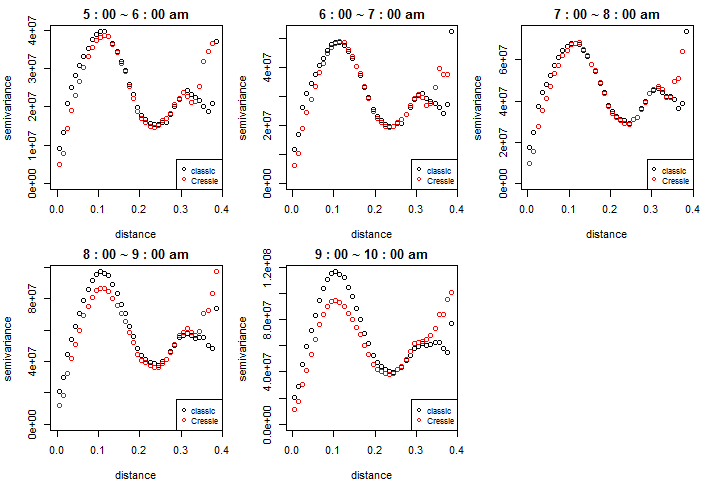
\includegraphics[width=\textwidth]{semi.png}
		\caption{Semivariogram with Classical and Cressie Weight \label{fig:semi}}
	\end{figure}
	Figure \ref{fig:semi} shows the semivariogram by time. There is obvious difference between the classical and Cressie weights, especially in 8-9 and 9-10 time period. As the scale is quite large, the difference is severe. Since Cressie weight is more robust, which can also be seen from plots, Cressie weight is used in the analysis.
	\begin{figure}[!ht]
		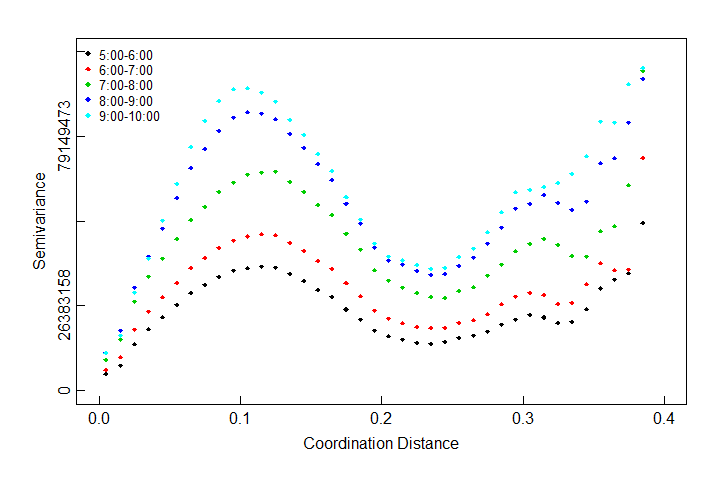
\includegraphics[width=\textwidth]{semi_full.png}
		\caption{Semivariogram with All Time in One \label{fig:semi_one}}
	\end{figure}
	Figure \ref{fig:semi_one} further convinces our induction in Section \ref{sec:meth} in that the semivariogram becomes decreasing after 0.1. We select 0.15 as our largest distance in further analysis as 0.15 corresponding to a roughly 14km. In addition, Figure \ref{fig:semi_one} also shows that the variance is increasing by time. The curves are more steady in earlier times while change severely at later times. This implies a trend from homogeneity to heterogeneity.
	
	\subsubsection{Semivario Fitting}
	Next, we try to capture the behavior of semivariogram within 0.15 distance by fitting semivariogram models. Cressie weight is applied while 8 covariance matrices are considered: spherical, exponential, Gaussian, cubic, Matern, circular, power and power.exponential. The corresponding estimates of parameters with residual sum of squares are listed in Tables in Appendix \ref{sec:appb}. Table \ref{tbl:compsem} lists the residual sum of squares of the eight models in different time slots. The last column calculates the mean residual of different time for each model. Based on the result, we can see the best model with smallest residual sum of squares is the Spherical model. The results are shown in Table \ref{semsph}. The practical range is around 0.1, which is smaller than 0.15, our choice of maximum distance.
	% latex table generated in R 3.3.1 by xtable 1.8-2 package
	% Mon Dec 05 23:55:04 2016
	\begin{table}[ht]
		\centering
		\caption{Comparison Between Different Semivariogram Models \label{tbl:compsem}}
		\begin{tabular}{rrrrrrr}
			\hline
			& 5 & 6 & 7 & 8 & 9 & mean \\ 
			\hline
			Spherical & 1345.8285 & 1492.5117 & 1584.2604 & 1087.8530 & 1313.3275 & 1364.7562 \\ 
			Exponential & 1784.8855 & 1777.4990 & 1737.4838 & 1778.2459 & 2688.8343 & 1953.3897 \\ 
			Gaussian & 1585.4945 & 1768.0713 & 1850.2990 & 1292.0789 & 1369.6244 & 1573.1136 \\ 
			Cubic & 1564.8268 & 1744.1053 & 1826.2688 & 1236.8298 & 1278.8814 & 1530.1824 \\ 
			Matern & 1784.8855 & 1777.4990 & 1737.4838 & 1778.2459 & 2688.8343 & 1953.3897 \\ 
			Circular & 1388.7989 & 1544.0794 & 1635.9566 & 1082.5673 & 1200.9239 & 1370.4652 \\ 
			Power & 4369.2902 & 4148.1227 & 3914.7066 & 4643.6822 & 6112.1596 & 4637.5923 \\ 
			Powered.exponential & 3177.1008 & 3017.0725 & 2784.1867 & 3302.9481 & 4695.4287 & 3395.3474 \\ 
			\hline
		\end{tabular}
	\end{table}

	\subsubsection{Likelihood Fitting}
	Likelihood fitting method is conducted in a similar way. Five covariance models: spherical, exponential, Gaussian, cubic and Matern are considered. Estimations with AIC and BIC for each model are listed in tables in Appendix \ref{sec:appb}. Table \ref{tbl:complik} summarizes the AIC and BIC for each model at different time with a mean at the last column. The smallest AIC and BIC models are exponential and Matern models, which have exactly the same results. The practical range is also around 0.1, less than 0.15.
	% latex table generated in R 3.3.1 by xtable 1.8-2 package
	% Tue Dec 06 00:29:43 2016
	\begin{table}[ht]
		\centering
		\caption{Comparison Between Different Likelihood Models \label{tbl:complik}}
		\begin{tabular}{rrrrrrr}
			\hline
			& 5 & 6 & 7 & 8 & 9 & mean \\ 
			\hline
			Spherical AIC & 4132.6943 & 4342.5478 & 4689.4731 & 4830.2513 & 4771.8406 & 4553.3614 \\ 
			Exponential AIC & 4108.0388 & 4315.9060 & 4659.6106 & 4805.0298 & 4756.6708 & 4529.0512 \\ 
			Gaussian AIC & 4859.8724 & 5033.1905 & 5318.4163 & 5550.9594 & 5661.5423 & 5284.7962 \\ 
			Cubic AIC & 4123.6046 & 4336.6447 & 4684.5895 & 4854.4454 & 4831.2214 & 4566.1011 \\ 
			Matern AIC & 4108.0388 & 4315.9060 & 4659.6106 & 4805.0298 & 4756.6708 & 4529.0512 \\ 
			Spherical BIC & 4151.3520 & 4361.2055 & 4708.1308 & 4848.9089 & 4790.4983 & 4572.0191 \\ 
			Exponential BIC & 4126.6964 & 4334.5636 & 4678.2683 & 4823.6874 & 4775.3285 & 4547.7088 \\ 
			Gaussian BIC & 4878.5301 & 5051.8482 & 5337.0739 & 5569.6170 & 5680.1999 & 5303.4538 \\ 
			Cubic BIC & 4142.2623 & 4355.3024 & 4703.2471 & 4873.1031 & 4849.8790 & 4584.7588 \\ 
			Matern BIC & 4126.6964 & 4334.5636 & 4678.2683 & 4823.6874 & 4775.3285 & 4547.7088 \\ 
			\hline
		\end{tabular}
	\end{table}
	
	\subsubsection{Effects of Covariates}
	Afterwards, we study the effects of covariates on frequency. Figure \ref{fig:disme} and Figure \ref{fig:disex} show the relationship of frequency on the two covariates over time.
	\begin{figure}[!ht]
		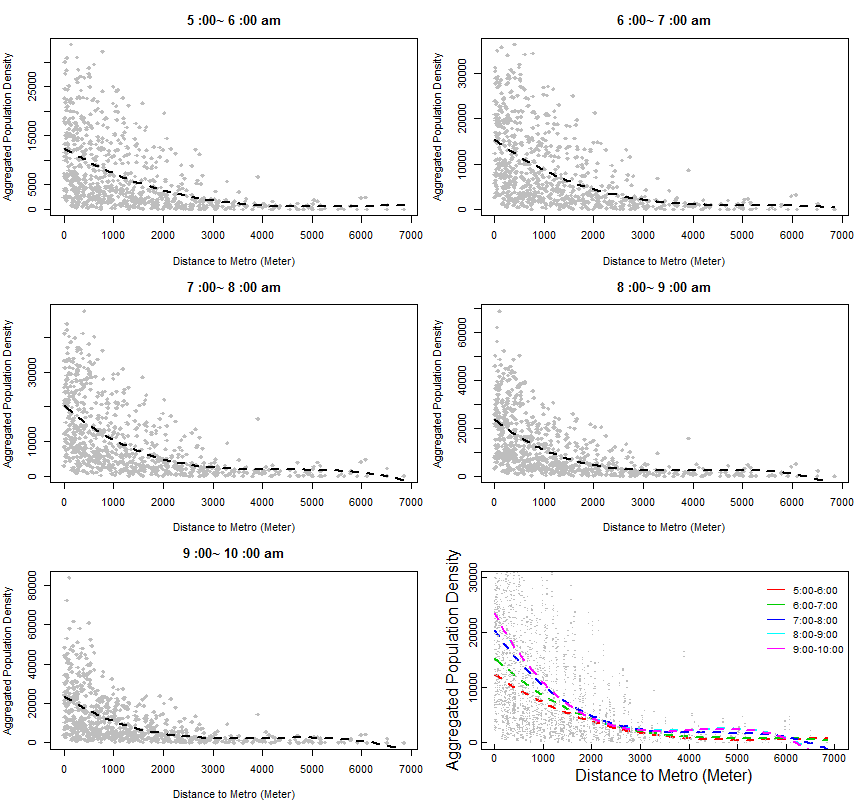
\includegraphics[width=\textwidth]{dist2metro.png}
		\caption{Relationship of Frequency on Distance2Metro \label{fig:disme}}
	\end{figure}
	\begin{figure}[!ht]
		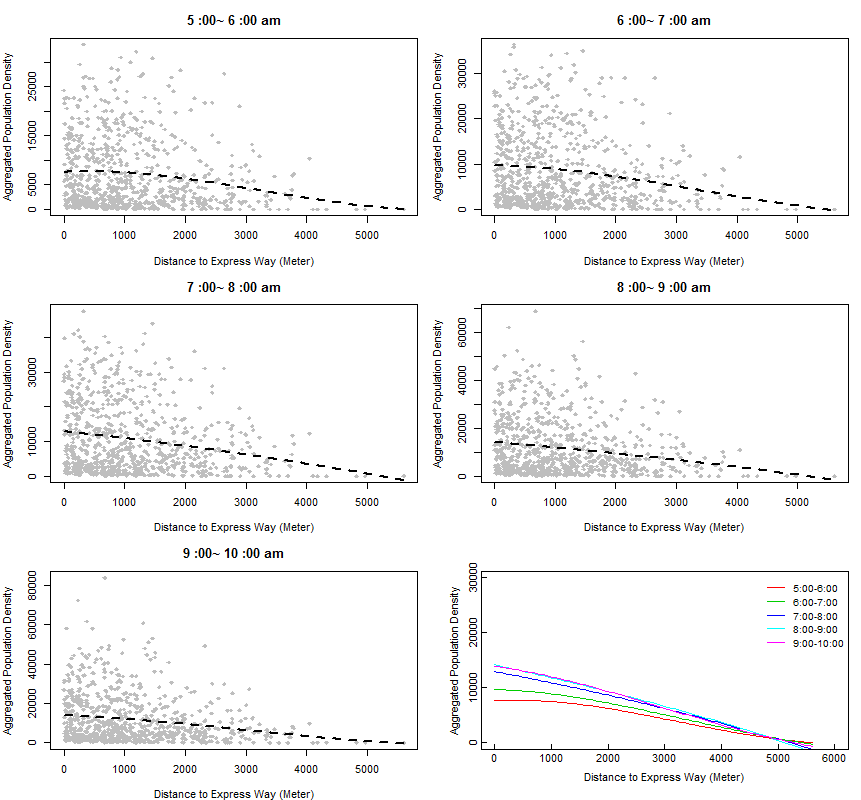
\includegraphics[width=\textwidth]{dist2express.png}
		\caption{Relationship of Frequency on Distance2Expressway \label{fig:disex}}
	\end{figure}
	
	Distances to transportation corridors have impact on population density with the smaller the distance, the larger the density. Also, as time increases, the population density also increases and the increase is more concentrated with shorter distances. Thus we conclude that the closer to transportation corridors, the more people. In addition, as time goes by, more people are gathering towards the metros or expressways.
	
	As shown in Section \ref{sec:reseda}, the frequency variable does not follow normal distribution, so a generalized model is considered. The histogram in Figure \ref{fig:hist} shows that a Gamma distribution seems appropriate for frequency. Also, the frequency, or density variable can be treated as count data due to our data aggregation method with disperse variance. Thus negative binomial family is also considered. For both with and without spatial effects model, we start with full quadratic terms. AIC is used in model selection. For GLM model with negative binomial family, AIC is not available. Thus residual sum of squares is compared to GLM model with Gamma family and the Gamma family has a much smaller residual sum of squares. After all comparisons, the best model is GAM model with spatial effect using Gamma family. Results are shown in Table \ref{tbl:bestx}. Results for other models are shown in Appendix \ref{sec:appb}.	
	% latex table generated in R 3.3.1 by xtable 1.8-2 package
	% Tue Dec 06 00:52:14 2016
	\begin{table}[ht]
		\centering
		\caption{Summary for Gamma GAM Spatial Model \label{tbl:bestx}}
		\begin{tabular}{rrrrr}
			\hline
			& Estimate & Std. Error & t value & Pr($>$$|$t$|$) \\ 
			\hline
			(Intercept) & 0.00 & 0.00 & 44.06 & 0.00 \\ 
			D2Metro & 0.00 & 0.00 & 1.51 & 0.13 \\ 
			D2Road & -0.00 & 0.00 & -2.57 & 0.01 \\ 
			I(D2Metro\verb|^|2) & 0.00 & 0.00 & 3.88 & 0.00 \\ 
			D2Metro:D2Road & 0.00 & 0.00 & 2.30 & 0.02 \\ 
			\hline
		\end{tabular}
	\end{table}
=======
	Histograms show that frequency is highly skewed. However, after log transformation, the histograms are still not desirable (shown in Figure \ref{fig:lghist}). Similarly, boxplot and qqplot also show that variable frequency does not follow normal distribution. After log transformation, it is still not normally distributed.
>>>>>>> origin/master

	Most of the coefficients are significant, further indicating that the covariates have impact on population density. The impact is huge since the parameter estimations are very close to zero because Gamma family uses inverse link. Results from model further prove previous conclusions from visualization.
	
	\subsection{Prediction}
	For visualization, we only present a comparison of true image with predicted images at 5:00 - 6:00 am, shown in Figure \ref{fig:pred5}. Residual sum of squares are compared at all time periods (Figure \ref{fig:predsum}).
	\begin{figure}[!ht]
		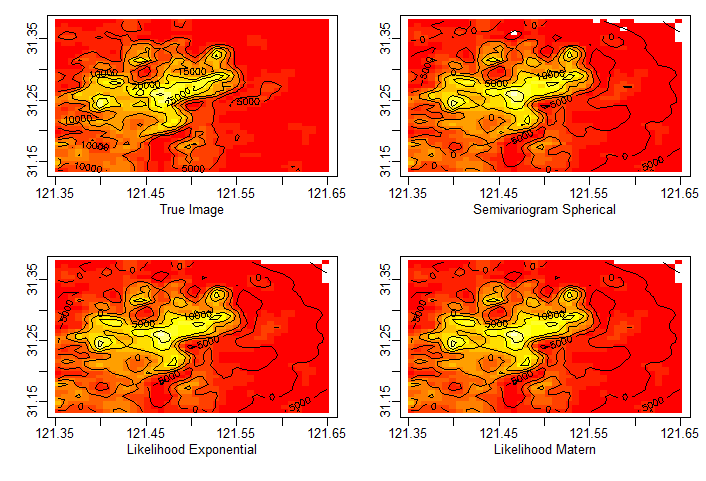
\includegraphics[width=\textwidth]{prediction_at_5.png}
		\caption{Comparison between True Model and Predicted Models \label{fig:pred5}}
	\end{figure}
	\begin{figure}[!ht]
		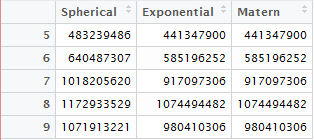
\includegraphics[width=\textwidth]{pred_result_total.png}
		\caption{Summary of Residual Sum of Squares between True Model and Predicted Models \label{fig:predsum}}
	\end{figure}

	 Although in each individual fitting, empirical methods fit better than likelihood fitting (see Figure \ref{fig:semsph} and Figure \ref{fig:likexp} in Appendix), for predicted models, the likelihood models are better than empirical fittings.
	 \begin{figure}[!ht]
	 	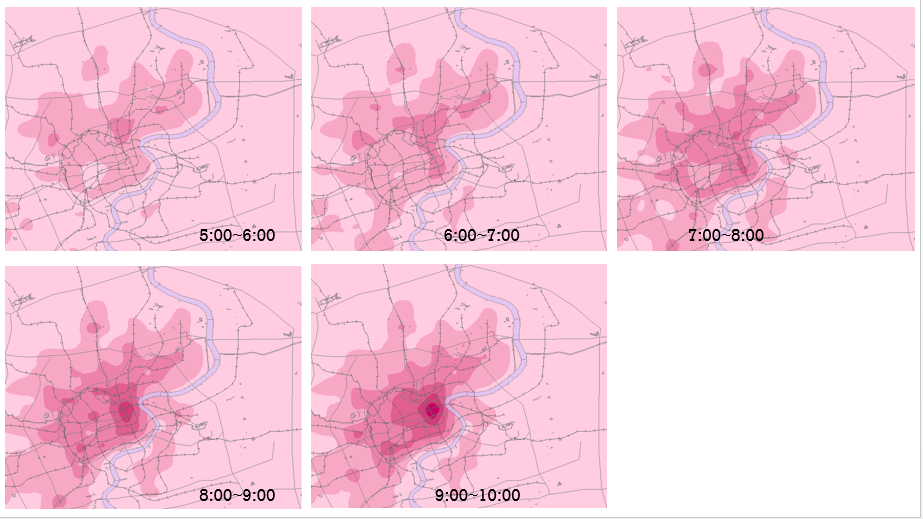
\includegraphics[width=\textwidth]{pred_exp.png}
	 	\caption{Predictions with Exponential Likelihood Models by Hour \label{fig:predexp}}
	 \end{figure}
 
	 Figure \ref{fig:predexp} displays predictions over time from likelihood fitted models with exponential covariance. It is clear that population movement is along transportation corridors.

	\section{Conclusion}\label{sec:con}
	This paper analyzes population movement in Shanghai during morning peak hours on a typical weekday using point-referenced data models in spatial analysis. Based on our study, especially the prediction plots, we have several findings:
	\begin{itemize}
		\item People are gathering towards CBD area by time;
		\item As time goes by, population density becomes more various;
		\item The closer to transportation corridors, the more people gathering;
		\item Increase in population is larger near metros or expressways;
		\item Population movement in along transportation corridors.
	\end{itemize}

	Due to time limitation, this report still has room for improvement.
	\begin{itemize}
		\item First, we also did areal analyses but did not finish it. We could conducted areal analysis and then compare the results with geostatistical analysis.
		\item Second, we can repeat the whole process for residuals from model with covariates. That is, the detrend model can include covariates.
		\item Third, we should also consider Bayesian models and then compare between the results.
		\item Fourth, a spatio-temporal model may be considered instead of looking at the trend by time from plots.
		\item Fifth, When making predictions, a leave-one-out cross validation may be applied to get a more accurate prediction.
	\end{itemize}
	
	\section{Reference}\label{sec:ref}
	\bibliography{sample}
	
	\clearpage
	\appendix
	\section{Appendices -- Plots} \label{sec:appa}
	\begin{figure}[!ht]
		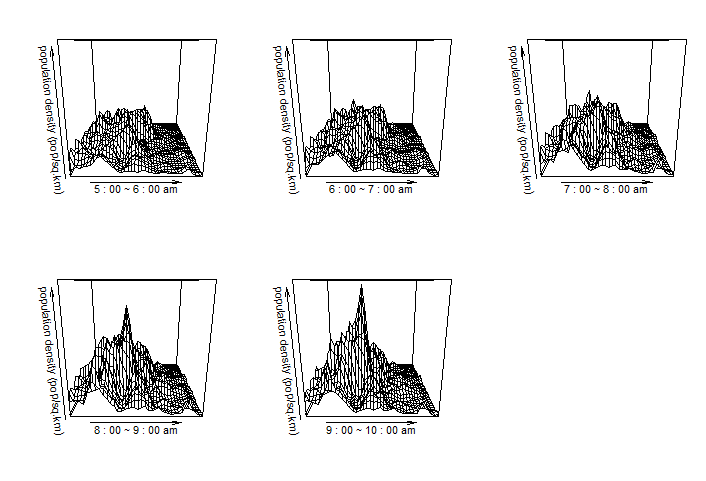
\includegraphics[width=\textwidth]{persp.png}
		\caption{Perspective Plot of Frequency by Hour \label{fig:perp}}
	\end{figure}
	\begin{figure}[!ht]
		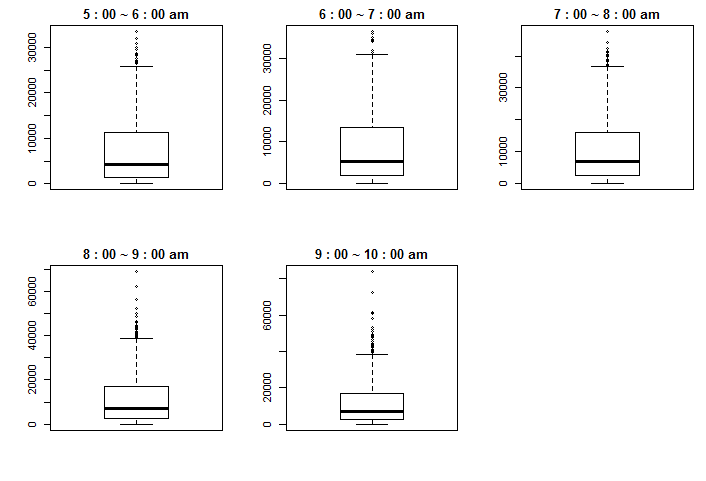
\includegraphics[width=\textwidth]{box.png}
		\caption{Boxplots of Frequency by Hour \label{fig:boxplot}}
<<<<<<< HEAD
	\end{figure}
	\begin{figure}[!ht]
		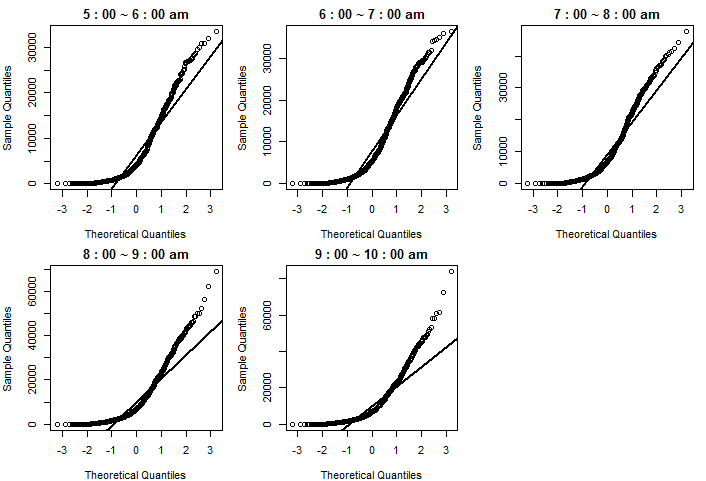
\includegraphics[width=\textwidth]{qq.png}
		\caption{QQ-Plots of Frequency by Hour \label{fig:qq}}
=======
	\end{figure}
	\begin{figure}[!ht]
		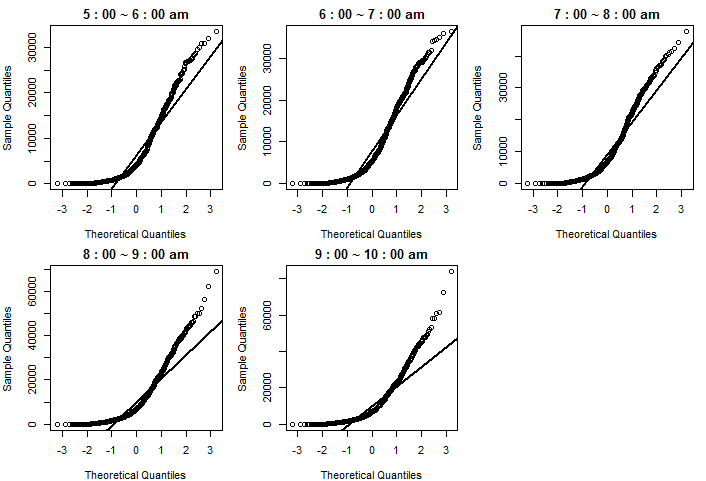
\includegraphics[width=\textwidth]{qq.png}
		\caption{QQ-Plots of Frequency by Hour \label{fig:qq}}
	\end{figure}
	\begin{figure}[!ht]
		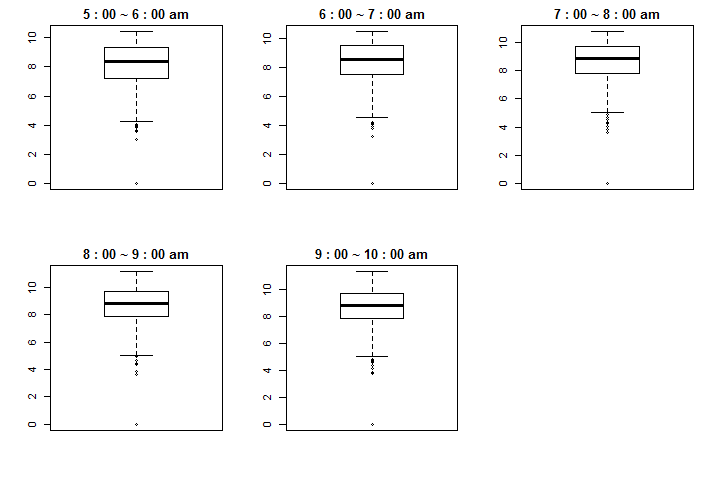
\includegraphics[width=\textwidth]{box_log.png}
		\caption{Boxplots of log-Frequency by Hour \label{fig:lgboxplot}}
	\end{figure}
	\begin{figure}[!ht]
		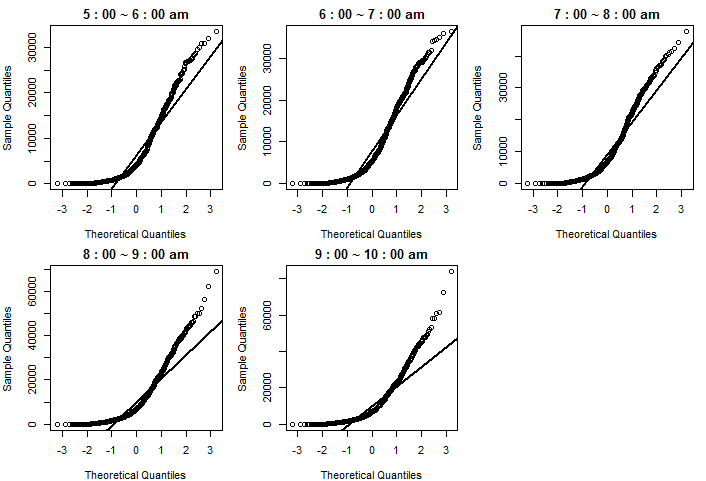
\includegraphics[width=\textwidth]{qq.png}
		\caption{QQ-Plots of log-Frequency by Hour \label{fig:lgqq}}
>>>>>>> origin/master
	\end{figure}
	\begin{figure}[!ht]
		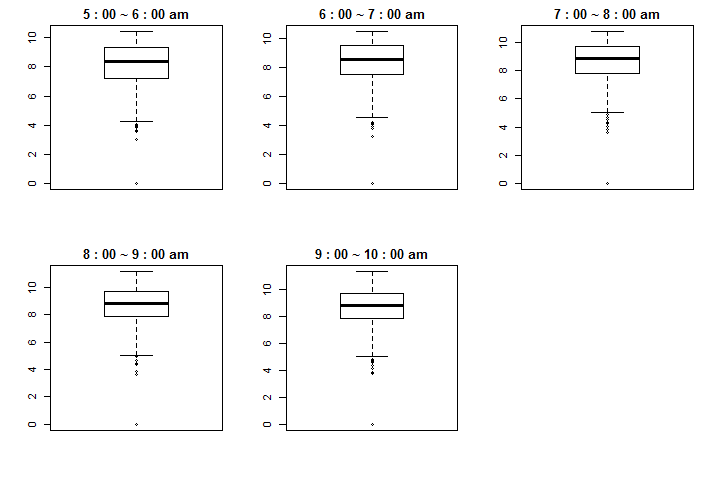
\includegraphics[width=\textwidth]{box_log.png}
		\caption{Boxplots of log-Frequency by Hour \label{fig:lgboxplot}}
	\end{figure}
	\begin{figure}[!ht]
		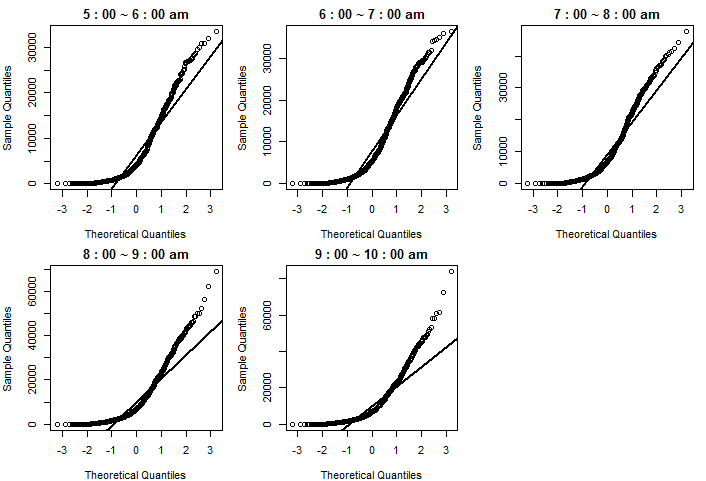
\includegraphics[width=\textwidth]{qq.png}
		\caption{QQ-Plots of log-Frequency by Hour \label{fig:lgqq}}
	\end{figure}
	\begin{figure}[!ht]
		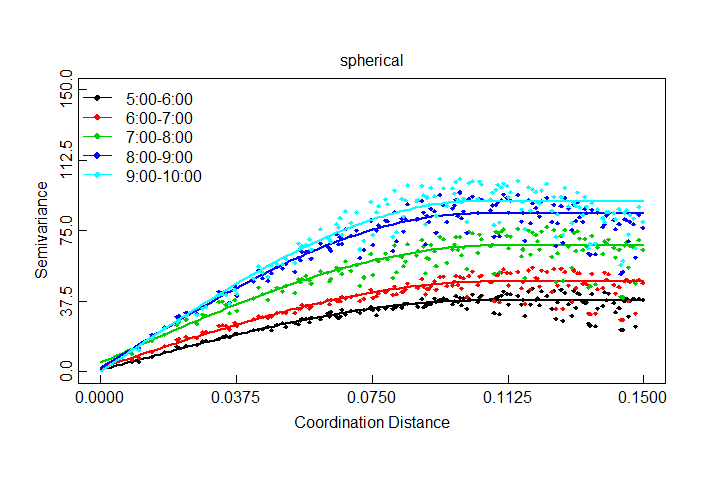
\includegraphics[width=\textwidth]{semfit_spherical.png}
		\caption{Empirical Fitted Model with Spherical Covariance \label{fig:semsph}}
	\end{figure}
	\begin{figure}[!ht]
		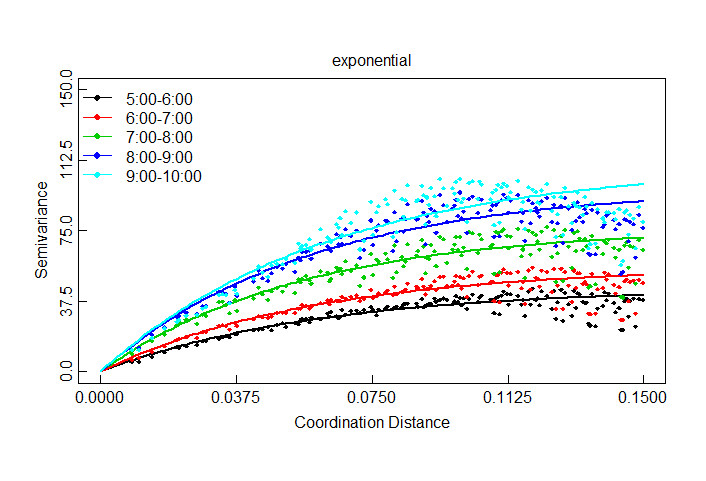
\includegraphics[width=\textwidth]{semfit_exponential.png}
		\caption{Empirical Fitted Model with Exponential Covariance \label{fig:semexp}}
	\end{figure}
	\begin{figure}[!ht]
		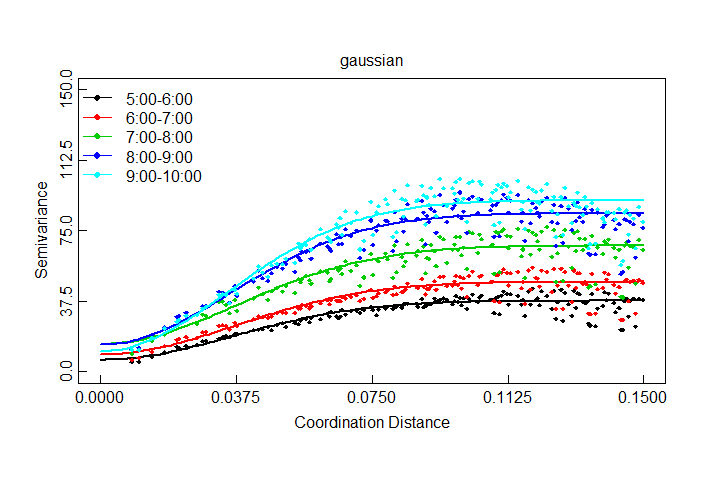
\includegraphics[width=\textwidth]{semfit_gaussian.png}
		\caption{Empirical Fitted Model with Gaussian Covariance \label{fig:semgau}}
	\end{figure}
	\begin{figure}[!ht]
		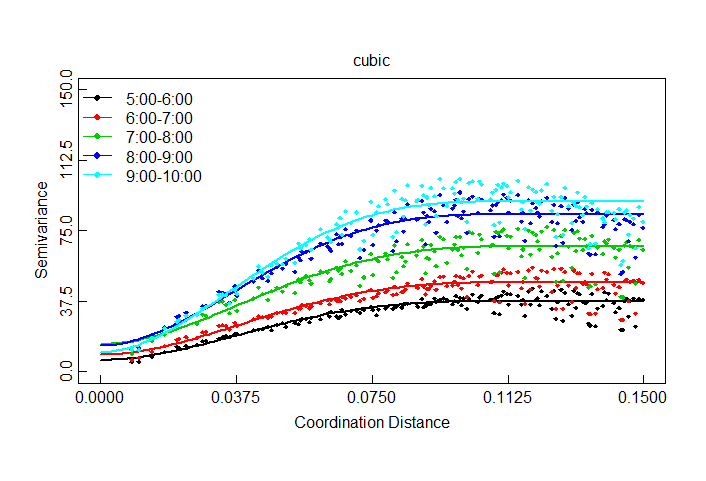
\includegraphics[width=\textwidth]{semfit_cubic.png}
		\caption{Empirical Fitted Model with Cubic Covariance \label{fig:semcub}}
	\end{figure}
	\begin{figure}[!ht]
		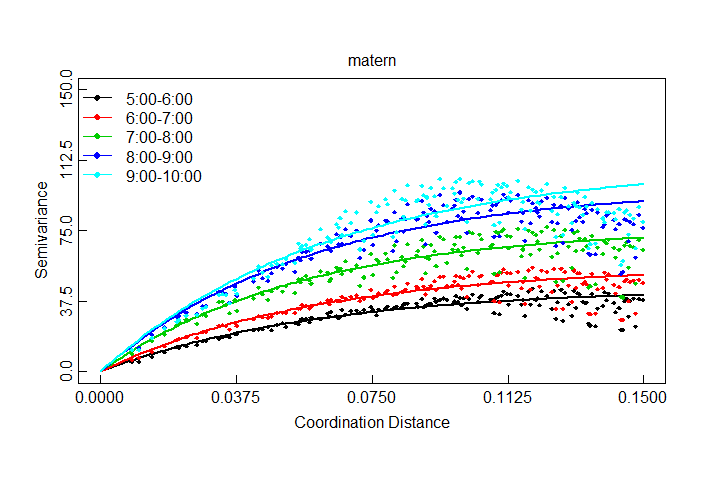
\includegraphics[width=\textwidth]{semfit_matern.png}
		\caption{Empirical Fitted Model with Matern Covariance \label{fig:semmat}}
	\end{figure}
	\begin{figure}[!ht]
		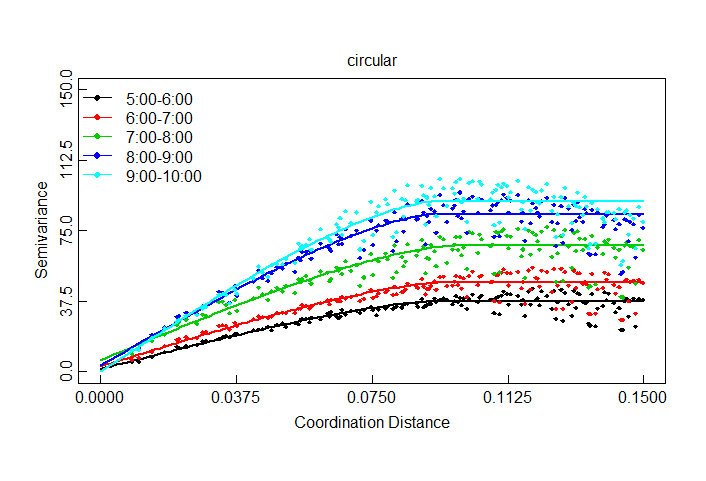
\includegraphics[width=\textwidth]{semfit_circular.png}
		\caption{Empirical Fitted Model with Circular Covariance \label{fig:semcirh}}
	\end{figure}
	\begin{figure}[!ht]
		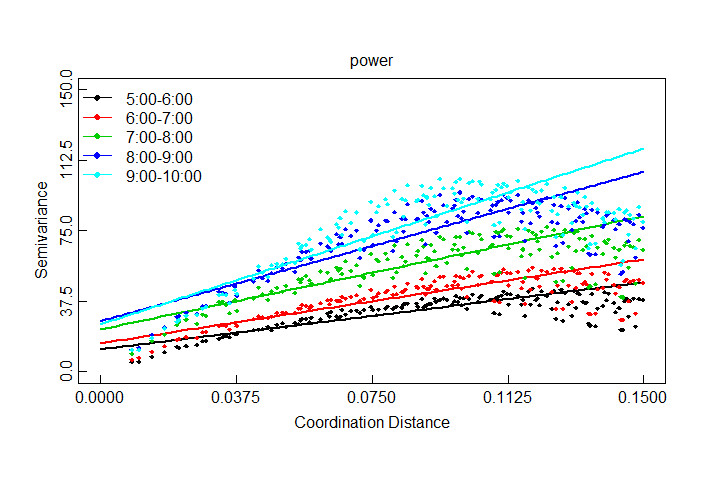
\includegraphics[width=\textwidth]{semfit_power.png}
		\caption{Empirical Fitted Model with Power Covariance \label{fig:sempow}}
	\end{figure}
	\begin{figure}[!ht]
		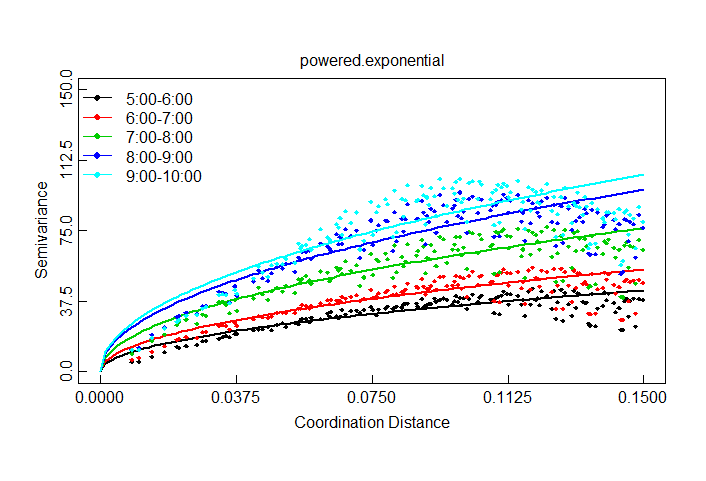
\includegraphics[width=\textwidth]{semfit_poweredexp.png}
		\caption{Empirical Fitted Model with Power Exponential Covariance \label{fig:sempex}}
	\end{figure}
	\begin{figure}[!ht]
		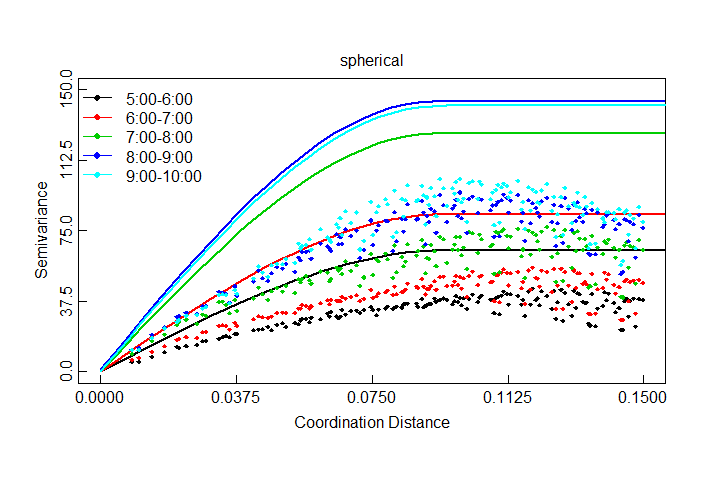
\includegraphics[width=\textwidth]{lik_spherical.png}
		\caption{Likelihood Fitted Model with Spherical Covariance \label{fig:liksph}}
	\end{figure}
	\begin{figure}[!ht]
		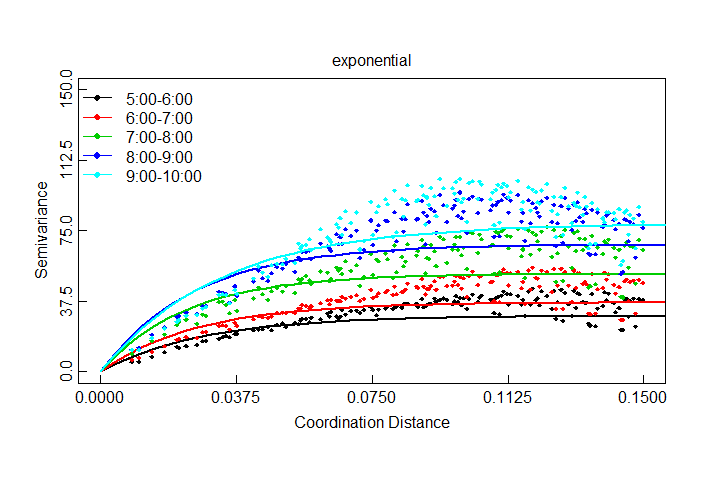
\includegraphics[width=\textwidth]{lik_exponential.png}
		\caption{Likelihood Fitted Model with Exponential Covariance \label{fig:likexp}}
	\end{figure}
	\begin{figure}[!ht]
		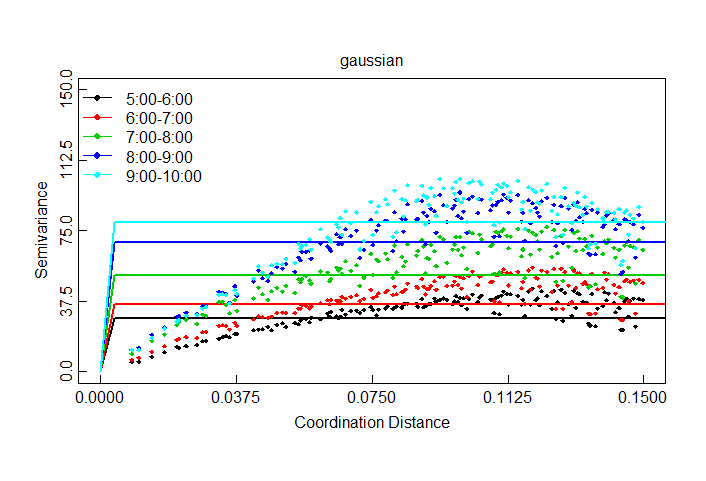
\includegraphics[width=\textwidth]{lik_gaussian.png}
		\caption{Likelihood Fitted Model with Gaussian Covariance \label{fig:likgau}}
	\end{figure}
	\begin{figure}[!ht]
		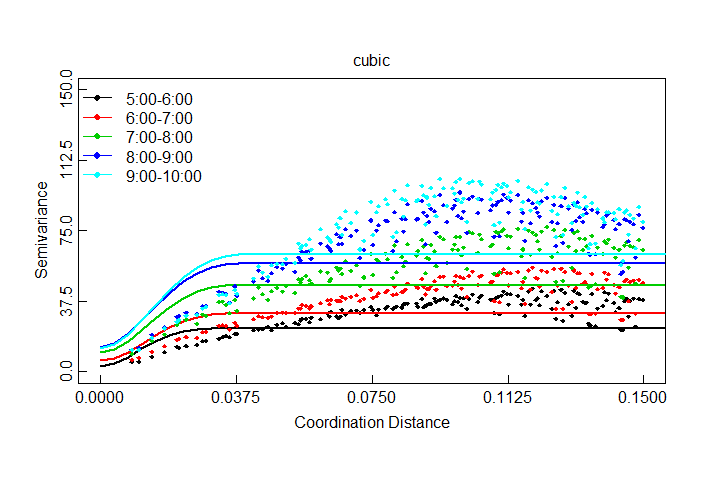
\includegraphics[width=\textwidth]{lik_cubic.png}
		\caption{Likelihood Fitted Model with Cubic Covariance \label{fig:likcub}}
	\end{figure}
	\begin{figure}[!ht]
		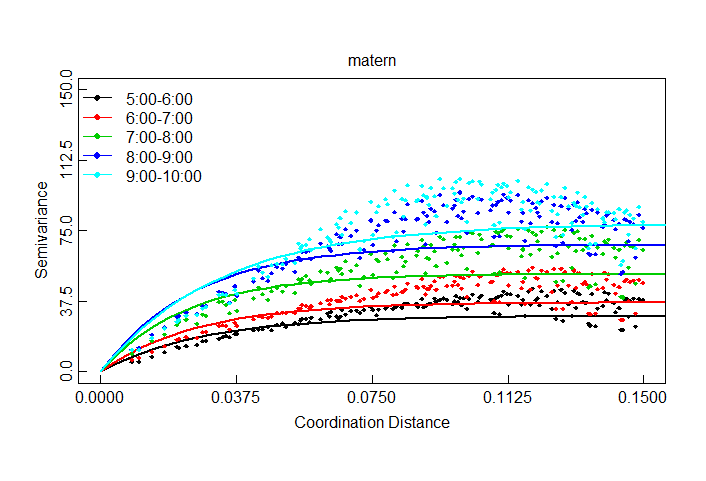
\includegraphics[width=\textwidth]{lik_matern.png}
		\caption{Likelihood Fitted Model with Matern Covariance \label{fig:likmat}}
	\end{figure}
	

	
	\clearpage
	\section{Appendices -- Tables} \label{sec:appb}
	% latex table generated in R 3.3.1 by xtable 1.8-2 package
	% Mon Dec 05 23:37:20 2016
	% latex table generated in R 3.3.1 by xtable 1.8-2 package
	% Tue Dec 06 02:05:41 2016
	\begin{table}[!ht]
		\centering
		\caption{Model Fitting for Trend Analysis at 5:00-6:00 am \label{tbl:trend5}}
		\begin{tabular}{rrrrr}
			\hline
			& Estimate & Std. Error & t value & Pr($>$$|$t$|$) \\ 
			\hline
			(Intercept) & -4524276582.8114 & 424064294.7508 & -10.67 & 0.0000 \\ 
			long & 69322413.3717 & 6759171.6736 & 10.26 & 0.0000 \\ 
			lat & 20175470.1376 & 4428300.0819 & 4.56 & 0.0000 \\ 
			I(long\verb|^|2) & -301768.0425 & 27548.8416 & -10.95 & 0.0000 \\ 
			I(lat\verb|^|2) & -569845.3908 & 40615.1361 & -14.03 & 0.0000 \\ 
			long:lat & 127051.1352 & 29861.1852 & 4.25 & 0.0000 \\ 
			\hline
		\end{tabular}
	\end{table}
	% latex table generated in R 3.3.1 by xtable 1.8-2 package
	% Tue Dec 06 02:07:06 2016
	\begin{table}[!ht]
		\centering
		\caption{Model Fitting for Trend Analysis at 6:00-7:00 am \label{tbl:trend6}}
		\begin{tabular}{rrrrr}
			\hline
			& Estimate & Std. Error & t value & Pr($>$$|$t$|$) \\ 
			\hline
			(Intercept) & -5407510455.9421 & 473626761.5300 & -11.42 & 0.0000 \\ 
			long & 83737786.8240 & 7549149.1031 & 11.09 & 0.0000 \\ 
			lat & 20687688.3375 & 4945857.1562 & 4.18 & 0.0000 \\ 
			I(long\verb|^|2) & -365755.1095 & 30768.6093 & -11.89 & 0.0000 \\ 
			I(lat\verb|^|2) & -648193.1651 & 45362.0255 & -14.29 & 0.0000 \\ 
			long:lat & 163098.1812 & 33351.2079 & 4.89 & 0.0000 \\ 
			\hline
		\end{tabular}
	\end{table}
	% latex table generated in R 3.3.1 by xtable 1.8-2 package
	% Tue Dec 06 02:07:42 2016
	\begin{table}[!ht]
		\centering
		\caption{Model Fitting for Trend Analysis at 7:00-8:00 am \label{tbl:trend7}}
		\begin{tabular}{rrrrr}
			\hline
			& Estimate & Std. Error & t value & Pr($>$$|$t$|$) \\ 
			\hline
			(Intercept) & -6797792159.1983 & 568114946.2249 & -11.97 & 0.0000 \\ 
			long & 106613345.8914 & 9055198.7031 & 11.77 & 0.0000 \\ 
			lat & 20773635.1185 & 5932551.9597 & 3.50 & 0.0005 \\ 
			I(long\verb|^|2) & -468492.8066 & 36906.9239 & -12.69 & 0.0000 \\ 
			I(lat\verb|^|2) & -779116.2191 & 54411.7157 & -14.32 & 0.0000 \\ 
			long:lat & 229656.4017 & 40004.7489 & 5.74 & 0.0000 \\ 
			\hline
		\end{tabular}
	\end{table}
	% latex table generated in R 3.3.1 by xtable 1.8-2 package
	% Tue Dec 06 02:08:33 2016
	\begin{table}[!ht]
		\centering
		\caption{Model Fitting for Trend Analysis at 8:00-9:00 am \label{tbl:trend8}}
		\begin{tabular}{rrrrr}
			\hline
			& Estimate & Std. Error & t value & Pr($>$$|$t$|$) \\ 
			\hline
			(Intercept) & -7808786493.0229 & 658937904.9085 & -11.85 & 0.0000 \\ 
			long & 122155012.8002 & 10502828.1716 & 11.63 & 0.0000 \\ 
			lat & 25071716.4924 & 6880972.5657 & 3.64 & 0.0003 \\ 
			I(long\verb|^|2) & -539521.6274 & 42807.1313 & -12.60 & 0.0000 \\ 
			I(lat\verb|^|2) & -954608.3493 & 63110.3656 & -15.13 & 0.0000 \\ 
			long:lat & 284515.5742 & 46400.1970 & 6.13 & 0.0000 \\ 
			\hline
		\end{tabular}
	\end{table}
	% latex table generated in R 3.3.1 by xtable 1.8-2 package
	% Tue Dec 06 02:09:11 2016
	\begin{table}[!ht]
		\centering
		\caption{Model Fitting for Trend Analysis at 9:00-10:00 am \label{tbl:trend9}}
		\begin{tabular}{rrrrr}
			\hline
			& Estimate & Std. Error & t value & Pr($>$$|$t$|$) \\ 
			\hline
			(Intercept) & -7974065064.3337 & 707087303.4041 & -11.28 & 0.0000 \\ 
			long & 124648083.4399 & 11270282.6696 & 11.06 & 0.0000 \\ 
			lat & 25962272.8934 & 7383773.6455 & 3.52 & 0.0005 \\ 
			I(long\verb|^|2) & -551936.4121 & 45935.1007 & -12.02 & 0.0000 \\ 
			I(lat\verb|^|2) & -1001344.2093 & 67721.9172 & -14.79 & 0.0000 \\ 
			long:lat & 301227.1079 & 49790.7161 & 6.05 & 0.0000 \\ 
			\hline
		\end{tabular}
	\end{table}
	\begin{table}[!ht]
		\centering
		\caption{Semivariogram Fitting with Spherical Covariance \label{semsph}}
		\begin{tabular}{rrrrrr}
			\hline
			& nugget & sigma.sq & phi & range & sum.of.sq \\ 
			\hline
			5 & 0.80 & 36.98 & 0.11 & 0.11 & 1345.83 \\ 
			6 & 1.95 & 45.93 & 0.11 & 0.11 & 1492.51 \\ 
			7 & 4.72 & 62.39 & 0.11 & 0.11 & 1584.26 \\ 
			8 & 1.96 & 82.11 & 0.10 & 0.10 & 1087.85 \\ 
			9 & 0.00 & 90.89 & 0.10 & 0.10 & 1313.33 \\ 
			\hline
		\end{tabular}
	\end{table}
	% latex table generated in R 3.3.1 by xtable 1.8-2 package
	% Mon Dec 05 23:42:41 2016
	\begin{table}[!ht]
		\centering
		\caption{Semivariogram Fitting with Exponential Covariance \label{semexp}}
		\begin{tabular}{rrrrrr}
			\hline
			& nugget & sigma.sq & phi & range & sum.of.sq \\ 
			\hline
			5 & 0.00 & 44.45 & 0.06 & 0.18 & 1784.89 \\ 
			6 & 0.00 & 55.70 & 0.06 & 0.18 & 1777.50 \\ 
			7 & 0.00 & 76.33 & 0.06 & 0.16 & 1737.48 \\ 
			8 & 0.00 & 97.93 & 0.06 & 0.17 & 1778.25 \\ 
			9 & 0.00 & 109.76 & 0.06 & 0.19 & 2688.83 \\ 
			\hline
		\end{tabular}
	\end{table}
	% latex table generated in R 3.3.1 by xtable 1.8-2 package
	% Mon Dec 05 23:43:19 2016
	\begin{table}[!ht]
		\centering
		\caption{Semivariogram Fitting with Gaussian Covariance \label{semgau}}
		\begin{tabular}{rrrrrr}
			\hline
			& nugget & sigma.sq & phi & range & sum.of.sq \\ 
			\hline
			5 & 6.28 & 31.44 & 0.05 & 0.09 & 1585.49 \\ 
			6 & 9.10 & 38.71 & 0.05 & 0.09 & 1768.07 \\ 
			7 & 14.73 & 52.33 & 0.05 & 0.09 & 1850.30 \\ 
			8 & 14.30 & 69.93 & 0.05 & 0.09 & 1292.08 \\ 
			9 & 10.85 & 80.29 & 0.05 & 0.09 & 1369.62 \\ 
			\hline
		\end{tabular}
	\end{table}
	% latex table generated in R 3.3.1 by xtable 1.8-2 package
	% Mon Dec 05 23:44:14 2016
	\begin{table}[!ht]
		\centering
		\caption{Semivariogram Fitting with Cubic Covariance \label{semcub}}
		\begin{tabular}{rrrrrr}
			\hline
			& nugget & sigma.sq & phi & range & sum.of.sq \\ 
			\hline
			5 & 6.19 & 31.38 & 0.12 & 0.12 & 1564.83 \\ 
			6 & 9.03 & 38.60 & 0.13 & 0.13 & 1744.11 \\ 
			7 & 14.67 & 52.14 & 0.13 & 0.13 & 1826.27 \\ 
			8 & 13.96 & 69.87 & 0.12 & 0.12 & 1236.83 \\ 
			9 & 10.35 & 80.26 & 0.12 & 0.12 & 1278.88 \\ 
			\hline
		\end{tabular}
	\end{table}
	% latex table generated in R 3.3.1 by xtable 1.8-2 package
	% Mon Dec 05 23:52:09 2016
	\begin{table}[!ht]
		\centering
		\caption{Semivariogram Fitting with Matern Covariance \label{semmat}}
		\begin{tabular}{rrrrrr}
			\hline
			& nugget & sigma.sq & phi & range & sum.of.sq \\ 
			\hline
			5 & 0.00 & 44.45 & 0.06 & 0.18 & 1784.89 \\ 
			6 & 0.00 & 55.70 & 0.06 & 0.18 & 1777.50 \\ 
			7 & 0.00 & 76.33 & 0.06 & 0.16 & 1737.48 \\ 
			8 & 0.00 & 97.93 & 0.06 & 0.17 & 1778.25 \\ 
			9 & 0.00 & 109.76 & 0.06 & 0.19 & 2688.83 \\ 
			\hline
		\end{tabular}
	\end{table}
	% latex table generated in R 3.3.1 by xtable 1.8-2 package
	% Mon Dec 05 23:52:52 2016
	\begin{table}[!ht]
		\centering
		\caption{Semivariogram Fitting with Circular Covariance \label{semcir}}
		\begin{tabular}{rrrrrr}
			\hline
			& nugget & sigma.sq & phi & range & sum.of.sq \\ 
			\hline
			5 & 1.41 & 36.27 & 0.09 & 0.09 & 1388.80 \\ 
			6 & 2.84 & 44.91 & 0.10 & 0.10 & 1544.08 \\ 
			7 & 6.13 & 60.85 & 0.10 & 0.10 & 1635.96 \\ 
			8 & 3.27 & 80.60 & 0.09 & 0.09 & 1082.57 \\ 
			9 & 0.00 & 90.52 & 0.09 & 0.09 & 1200.92 \\ 
			\hline
		\end{tabular}
	\end{table}
	% latex table generated in R 3.3.1 by xtable 1.8-2 package
	% Mon Dec 05 23:53:30 2016
	\begin{table}[!ht]
		\centering
		\caption{Semivariogram Fitting with Power Covariance \label{sempow}}
		\begin{tabular}{rrrrrr}
			\hline
			& nugget & sigma.sq & phi & range & sum.of.sq \\ 
			\hline
			5 & 11.80 & 238.28 & 1.00 & Inf & 4369.29 \\ 
			6 & 15.11 & 297.83 & 1.00 & Inf & 4148.12 \\ 
			7 & 22.54 & 401.87 & 1.00 & Inf & 3914.71 \\ 
			8 & 26.87 & 531.49 & 1.00 & Inf & 4643.68 \\ 
			9 & 25.26 & 623.86 & 1.00 & Inf & 6112.16 \\ 
			\hline
		\end{tabular}
	\end{table}
	% latex table generated in R 3.3.1 by xtable 1.8-2 package
	% Mon Dec 05 23:54:09 2016
	\begin{table}[!ht]
		\centering
		\caption{Semivariogram Fitting with Power Exponential Covariance \label{sempex}}
		\begin{tabular}{rrrrrr}
			\hline
			& nugget & sigma.sq & phi & range & sum.of.sq \\ 
			\hline
			5 & 0.00 & 1136.84 & 100.29 & 900.02 & 3177.10 \\ 
			6 & 0.00 & 1314.45 & 83.80 & 752.10 & 3017.07 \\ 
			7 & 0.00 & 1789.32 & 78.89 & 707.96 & 2784.19 \\ 
			8 & 0.00 & 2855.52 & 125.97 & 1130.48 & 3302.95 \\ 
			9 & 0.00 & 2885.65 & 109.40 & 981.77 & 4695.43 \\ 
			\hline
		\end{tabular}
	\end{table}
	% latex table generated in R 3.3.1 by xtable 1.8-2 package
	% Tue Dec 06 00:04:45 2016
	\begin{table}[!ht]
		\centering
		\caption{Likelihood Fitting with Spherical Covariance \label{tbl:liksph}}
		\begin{tabular}{rrrrrrr}
			\hline
			& nugget & sigma.sq & phi & range & AIC & BIC \\ 
			\hline
			5 & 0.00 & 64.72 & 0.10 & 0.10 & 4132.69 & 4151.35 \\ 
			6 & 0.00 & 83.96 & 0.10 & 0.10 & 4342.55 & 4361.21 \\ 
			7 & 0.00 & 126.83 & 0.09 & 0.09 & 4689.47 & 4708.13 \\ 
			8 & 1.01 & 143.01 & 0.09 & 0.09 & 4830.25 & 4848.91 \\ 
			9 & 0.00 & 141.49 & 0.09 & 0.09 & 4771.84 & 4790.50 \\ 
			\hline
		\end{tabular}
	\end{table}
	% latex table generated in R 3.3.1 by xtable 1.8-2 package
	% Tue Dec 06 00:09:58 2016
	\begin{table}[!ht]
		\centering
		\caption{Likelihood Fitting with Exponential Covariance \label{tbl:likexp}}
		\begin{tabular}{rrrrrrr}
			\hline
			& nugget & sigma.sq & phi & range & AIC & BIC \\ 
			\hline
			5 & 0.00 & 29.72 & 0.03 & 0.08 & 4108.04 & 4126.70 \\ 
			6 & 0.00 & 36.85 & 0.03 & 0.08 & 4315.91 & 4334.56 \\ 
			7 & 0.00 & 52.04 & 0.02 & 0.07 & 4659.61 & 4678.27 \\ 
			8 & 0.00 & 67.68 & 0.03 & 0.08 & 4805.03 & 4823.69 \\ 
			9 & 0.00 & 78.78 & 0.03 & 0.10 & 4756.67 & 4775.33 \\ 
			\hline
		\end{tabular}
	\end{table}
	% latex table generated in R 3.3.1 by xtable 1.8-2 package
	% Tue Dec 06 00:14:57 2016
	\begin{table}[!ht]
		\centering
		\caption{Likelihood Fitting with Gaussian Covariance \label{tbl:likgau}}
		\begin{tabular}{rrrrrrr}
			\hline
			& nugget & sigma.sq & phi & range & AIC & BIC \\ 
			\hline
			5 & 0.00 & 28.52 & 0.00 & 0.00 & 4859.87 & 4878.53 \\ 
			6 & 0.00 & 35.58 & 0.00 & 0.00 & 5033.19 & 5051.85 \\ 
			7 & 0.00 & 51.19 & 0.00 & 0.00 & 5318.42 & 5337.07 \\ 
			8 & 0.00 & 68.87 & 0.00 & 0.00 & 5550.96 & 5569.62 \\ 
			9 & 0.00 & 79.30 & 0.00 & 0.00 & 5661.54 & 5680.20 \\ 
			\hline
		\end{tabular}
	\end{table}
	% latex table generated in R 3.3.1 by xtable 1.8-2 package
	% Tue Dec 06 00:22:35 2016
	\begin{table}[!ht]
		\centering
		\caption{Likelihood Fitting with Cubic Covariance \label{tbl:likcub}}
		\begin{tabular}{rrrrrrr}
			\hline
			& nugget & sigma.sq & phi & range & AIC & BIC \\ 
			\hline
			5 & 2.80 & 20.05 & 0.03 & 0.03 & 4123.60 & 4142.26 \\ 
			6 & 5.78 & 25.24 & 0.04 & 0.04 & 4336.64 & 4355.30 \\ 
			7 & 10.16 & 35.98 & 0.04 & 0.04 & 4684.59 & 4703.25 \\ 
			8 & 13.12 & 44.67 & 0.04 & 0.04 & 4854.45 & 4873.10 \\ 
			9 & 12.18 & 50.48 & 0.05 & 0.05 & 4831.22 & 4849.88 \\ 
			\hline
		\end{tabular}
	\end{table}
	% latex table generated in R 3.3.1 by xtable 1.8-2 package
	% Tue Dec 06 00:27:58 2016
	\begin{table}[!ht]
		\centering
		\caption{Likelihood Fitting with Matern Covariance \label{tbl:likmat}}
		\begin{tabular}{rrrrrrr}
			\hline
			& nugget & sigma.sq & phi & range & AIC & BIC \\ 
			\hline
			5 & 0.00 & 29.72 & 0.03 & 0.08 & 4108.04 & 4126.70 \\ 
			6 & 0.00 & 36.85 & 0.03 & 0.08 & 4315.91 & 4334.56 \\ 
			7 & 0.00 & 52.04 & 0.02 & 0.07 & 4659.61 & 4678.27 \\ 
			8 & 0.00 & 67.68 & 0.03 & 0.08 & 4805.03 & 4823.69 \\ 
			9 & 0.00 & 78.78 & 0.03 & 0.10 & 4756.67 & 4775.33 \\ 
			\hline
		\end{tabular}
	\end{table}
	% latex table generated in R 3.3.1 by xtable 1.8-2 package
	% Tue Dec 06 00:40:48 2016
	\clearpage
	\begin{table}[!ht]
		\centering
		\caption{Gamma GLM with No Spatial Effect \label{tbl:gamglm}}
		\begin{tabular}{rrrrr}
			\hline
			& Estimate & Std. Error & t value & Pr($>$$|$t$|$) \\ 
			\hline
			(Intercept) & 0.0000 & 0.0000 & 15.52 & 0.0000 \\ 
			D2Metro & 0.0000 & 0.0000 & 4.82 & 0.0000 \\ 
			D2Road & -0.0000 & 0.0000 & -1.22 & 0.2236 \\ 
			I(D2Metro\verb|^|2) & 0.0000 & 0.0000 & 10.23 & 0.0000 \\ 
			I(D2Road\verb|^|2) & 0.0000 & 0.0000 & 3.08 & 0.0021 \\ 
			D2Metro:D2Road & 0.0000 & 0.0000 & 1.77 & 0.0768 \\ 
			\hline
		\end{tabular}
	\end{table}
	% latex table generated in R 3.3.1 by xtable 1.8-2 package
	% Tue Dec 06 01:04:42 2016
	\begin{table}[!ht]
		\centering
		\caption{Negative Binomial GLM with No Spatial Effect} \label{tbl:nbglm}
		\begin{tabular}{rrrrr}
			\hline
			& Estimate & Std. Error & t value & Pr($>$$|$t$|$) \\ 
			\hline
			(Intercept) & 9.6650 & 0.0412 & 234.76 & 0.0000 \\ 
			D2Metro & -0.0006 & 0.0000 & -15.83 & 0.0000 \\ 
			D2Road & 0.0004 & 0.0001 & 8.55 & 0.0000 \\ 
			I(D2Metro\verb|^|2) & 0.0000 & 0.0000 & 4.39 & 0.0000 \\ 
			I(D2Road\verb|^|2) & -0.0000 & 0.0000 & -7.79 & 0.0000 \\ 
			D2Metro:D2Road & -0.0000 & 0.0000 & -16.32 & 0.0000 \\ 
			\hline
		\end{tabular}
	\end{table}
	% latex table generated in R 3.3.1 by xtable 1.8-2 package
	% Tue Dec 06 01:05:32 2016
	\begin{table}[!ht]
		\centering
		\caption{Negative Binomial GAM with Spatial Effect} \label{tbl:nbgam}
		\begin{tabular}{rrrrr}
			\hline
			& Estimate & Std. Error & z value & Pr($>$$|$z$|$) \\ 
			\hline
			(Intercept) & 8.95 & 0.04 & 244.15 & 0.00 \\ 
			D2Metro & -0.00 & 0.00 & -8.68 & 0.00 \\ 
			D2Road & 0.00 & 0.00 & 7.33 & 0.00 \\ 
			I(D2Metro\verb|^|2) & 0.00 & 0.00 & 2.47 & 0.01 \\ 
			I(D2Road\verb|^|2) & -0.00 & 0.00 & -6.79 & 0.00 \\ 
			D2Metro:D2Road & -0.00 & 0.00 & -7.83 & 0.00 \\ 
			\hline
		\end{tabular}
	\end{table}


	\clearpage
	\section{Appendices -- R codes}
	\begin{verbatim}
		
	\end{verbatim}
	
\end{document}